\chapter{序列和字符串}
\label{chap:chapter4}
\minitoc

%\setcounter{lstlisting}{5}

在本章中,我们将开始编写Perl程序,来处理DNA和蛋白质的生物序列数据。在你的计算机上,一旦有了这样的序列,你就可以编写程序对序列数据进行下列的处理了:

\begin{itemize}
  \item 把DNA转录成RNA
  \item 把序列串联起来
  \item 获取反向互补序列
  \item 从文件中读取序列
\end{itemize}

此外,你还将编写获取序列信息的程序。DNA的GC含量如何?蛋白质的疏水性如何?你将学习相关的编程技术,利用它们就可以来回答这些类似的问题了。

在本章中你将学习到的技能涉及Perl语言的基础,此处列出了其中的一部分:

\begin{itemize}
  \item 标量变量
  \item 数组变量
  \item 替换、翻译等字符串的操作
  \item 从文件中读取数据
\end{itemize}

\section{序列数据的表征}
本书的大部分内容都是处理表征DNA和蛋白质生物学序列的符号。在生物信息学中,使用这些符号来表征序列,这些符号和生物学家日常工作中用来表征序列的符号是完全一样的。

如前所述,DNA是由四种基础分子组成的,它们就是核酸,也叫做核苷酸或碱基;而蛋白质则是由20中基础分子组成的,它们就是氨基酸,也叫做残基。蛋白质的片段叫做肽(即缩氨酸)。不管是DNA还是蛋白质,本质上都是多聚物,由构成它们的基础分子首尾相连而形成。所以,仅仅通过碱基或氨基酸序列就可以表征DNA或蛋白质的基本结构。

这些都是最基本的定义。我假设你对这些内容都比较熟悉,或者打算查阅一本入门性的参考书来学习更加详细的内容。\autoref{tab:table4.1}中列出的是碱基;在碱基上加上一个糖基,就可以得到核苷:腺苷、鸟苷、胞苷、胸苷和尿苷;在核苷上再加一个磷酸基团,就可以得到核苷酸:腺苷酸、鸟苷酸、胞苷酸、胸苷酸和尿苷酸。核酸就是由核苷酸通过化学键相连形成的序列。肽是由数个氨基酸相连而成的,更长的话就叫做多肽了。蛋白质是由一个或多个多肽组成的生物学功能基团。残基指的就是多肽链中的氨基酸。

为了方便,如\autoref{tab:table4.1}和\autoref{tab:table4.2}所示,常用一个字母或三个字母的代码来表示核酸和氨基酸。(本书中主要用单字母代码来表示氨基酸。)

\begin{table}[!htbp]
  \begin{center}
  \caption{标准的IUB/IUPAC核算代码}
  \label{tab:table4.1}
  %\begin{tabu}{X[1,c]X[2,l]}
  \begin{tabu} to 0.7\linewidth {X[1,c]X[2,c]}
  \toprule
  代码 & 核酸\\
  \midrule
  A & 腺嘌呤\\
  C & 胞嘧啶\\
  G & 鸟嘌呤\\
  T & 胸腺嘧啶\\
  U & 尿嘧啶\\
  M & A或C (aMino,氨基)\\
  R & A或G (puRine,嘌呤)\\
  W & A或T (Weak,作用力弱)\\
  S & C或G (Strong,作用力强)\\
  Y & C或T (pYrimidine,嘧啶)\\
  K & G或T (keto,酮基)\\
  V & A或C或G(非T)\\
  H & A或C或T(非G)\\
  D & A或G或T(非C)\\
  B & C或G或T(非A)\\
  N & A或G或C或T (aNy,任何一个碱基)\\
  \bottomrule
  \end{tabu}
  \end{center}
\end{table}

\autoref{tab:table4.1}中的核酸代码不仅包括四种基本核酸的字母缩写,还定义了二个核酸、三个核酸或四个核酸所有可能组合的单字母缩写。在本书的大多数例子中,我仅使用A、C、G、T、U和N。A、C、G和T字母代表了DNA的核酸,而当DNA(脱氧核糖核酸)转录成RNA(核糖核酸)时U将替换T。当测序仪无法确定碱基时,常用N来表示“未知碱基”。稍后,在\autoref{chap:chapter9}中,在编程处理限制性酶切图谱时,我们还需要用到表示各种核酸组合的其他代码。有时,也会使用这些单字母代码的小写形式,这对DNA来说比较常见,但在蛋白质中则很少这样使用。

\begin{table}[!htbp]
  \begin{center}
  \caption{标准的氨基酸代码}
  \label{tab:table4.2}
  %\begin{tabu}{X[1,c]X[2,l]}
  \begin{tabu} to \linewidth {X[1,c]X[2,c]X[1,c]}
  \toprule
  单字母代码 & 氨基酸 & 三字母代码\\
  \midrule
  A & Alanine,丙氨酸 & Ala\\
  B & Aspartic acid or Asparagine,天冬氨酸或天冬酰胺 & Asx\\
  C & Cysteine,半胱氨酸 & Cys\\
  D & Aspartic acid,天冬氨酸 &  Asp\\
  E & Glutamic acid,谷氨酸 & Glu\\
  F & Phenylalanine,苯丙氨酸 & Phe\\
  G & Glycine,甘氨酸 & Gly\\
  H & Histidine,组氨酸 & His\\
  I & Isoleucine,异亮氨酸 & Ile\\
  K & Lysine,赖氨酸 & Lys\\
  L & Leucine,亮氨酸 & Leu\\
  M & Methionine,甲硫氨酸 & Met\\
  N & Asparagine,天冬酰胺 & Asn\\
  P & Proline,脯氨酸 & Pro\\
  Q & Glutamine,谷氨酰胺 & Gln\\
  R & Arginine,精氨酸 & Arg\\
  S & Serine,丝氨酸 & Ser\\
  T & Threonine,苏氨酸 & Thr\\
  V & Valine,缬氨酸 & Val\\
  W & Tryptophan,色氨酸 & Trp\\
  X & Unknown,未知氨基酸 & Xxx\\
  Y & Tyrosine,酪氨酸 & Tyr\\
  Z & Glutamic acid or Glutamine,谷氨酸或谷氨酰胺 & Glx\\
  \bottomrule
  \end{tabu}
  \end{center}
\end{table}

对于\autoref{tab:table4.1}和\autoref{tab:table4.2}中的代码来说,计算机科学中的术语和生物学中的术语还是有一定差别的。从计算机科学的角度来看,这两个表定义了两个按字母顺序排列的有限的符号集合,使用它们可以来构建字符串。字符串指的就是符号序列。比如,这句话本身就是一个字符串(this sentence is a string)。语言就是一个(有限或无限)字符串的集合。在本书中,语言主要就是DNA和蛋白质的序列数据。和在序列数据中的具有生物学含义的表征不同,生物信息学家常常会把真正的DNA或蛋白质序列称作“字符串”。两个不同学科中的术语会交叉使用,这就是一个例子。

如同你在表格中看到的那样,我们会使用简单的字母来表征数据,这和在纸张上手写时使用的方式是一样的。计算机实际上会用另外的代码来表征简单的字母,但你不用担心这些,只要记住在使用文本编辑器时将它们保存为ASCII或者纯文本即可。

ASCII是计算机在内存中存储文本(和控制信息)数据的一种方式。当文本编辑器等程序读取数据时,计算机知道它正在读取ASCII,因为计算机知道每个代码代表什么,所以它就会在屏幕上以一种容易识别的方式把相应的母显示出来。总而言之,知道ASCII是计算机表征文本的一种代码就足够。\footnote{一种新的编码字符叫做Unicode,它可以表征世界上所有语言中的所有符号,因此现在已得到广泛使用,并且Perl对Unicode也有很好的支持。}

\section{存储DNA序列的程序}
让我们来写一个小程序吧,它把DNA存储在变量中,然后把它打印输出到屏幕上。我们会用最常用的方式——由A、C、G和T四个字母组成的字符串——来书写DNA,并且把存储DNA的变量叫做\verb|$DNA|。换言之,\verb|$DNA|就是程序中DNA序列数据的名称。注意这一点,在Perl中,变量就是你打算处理的数据的名称,使用该名称,你可以对数据进行完全的访问。\autoref{exam:example4.1}是完整的程序。

%\textbf{例4-1:把DNA存储到计算机中}
\lstinputlisting[label=exam:example4.1,caption={例4-1:把DNA存储到计算机中}]{./scripts/example4-1.pl}

在\autoref{chap:chapter2}中,我们已经学习了文本编辑器和运行Perl程序的知识,运用这些知识,输入例子中的代码(或者从书籍官网上把它复制下来)并保存到一个文件中。牢记一定要把程序保存成ASCII或者纯文本格式,否则Perl在读取该文件时可能会出现问题。

接下来就是运行程序了。运行程序的具体步骤取决于你使用的计算机(参看\autoref{chap:chapter2})。我们假定程序是你计算机中一个叫做\textit{example4-1}的文件。回顾\autoref{chap:chapter2}中相关的知识,如果你想在Unix或者Linux中运行这个程序,需要在shell窗口中键入:

\begin{lstlisting}[language=bash]
perl example4-1
\end{lstlisting}

在Mac中,使用MacPerl应用程序打开这个文件,并把它保存为droplet,然后双击该droplet即可。在Windows中,在MS-DOS命令窗口中键入:

\begin{lstlisting}[language=bash]
perl example4-1
\end{lstlisting}

如果你成功运行了该程序,在你的计算机屏幕上你将看到相应的输出。

\subsection{控制流}
\autoref{exam:example4.1}展示了所有Perl程序都将用到的许多理念,其中一个便是\textit{控制流}的理念,即计算机是以什么顺序来执行程序中的语句的。

所有的程序都从第一行开始,除非明确指明了其他的运行顺序,否则它将一条一条地执行语句,直到程序的最后一行。\autoref{exam:example4.1}只是简单的从头到尾执行程序,并没有其他的运行支路。

在后续的章节中,你将学习到如何编程控制程序的执行顺序。

\subsection{再说注释}
现在让我们看一下\autoref{exam:example4.1}程序中的细节。你会发现其中有许多空行,它们的存在使得程序更容易被人阅读。另外,注意以\#起始的注释。在\autoref{chap:chapter3}中提到过,当Perl运行时,它会把这些注释和空行全部忽略掉。事实上,对于Perl来说,下面的程序和\autoref{exam:example4.1}中的程序是完全一样的:

\begin{lstlisting}
#!/usr/bin/perl -w
$DNA = 'ACGGGAGGACGGGAAAATTACTACGGCATTAGC'; print $DNA; exit;
\end{lstlisting}

在\autoref{exam:example4.1}中,我使用了大量的注释。代码开始的注释指明了程序的用途、作者以及其他信息,但其他人需要理解代码时,这些信息会对他有很大的帮助。注释还解释了代码每一部分的作用,有时还对代码的工作原理进行了阐释。

了解注释的重要性是非常必要的。在大多数高校的计算机科学课程的课堂作业中,没有注释的程序通常会得到很低的分数甚至不及格;而在工作中不对代码进行注释的程序员,他的职业生涯将是短暂而失败的。

\subsection{命令解释}
\label{sec:section4.2.3}
程序的第一行以\#起始,这使得它看上去像是一行注释,但又不像是有什么信息含量的注释:

\begin{lstlisting}
#!/usr/bin/perl -w
\end{lstlisting}

这是比较特殊的一行,叫做命令解释,它告诉运行Unix或者Linux的计算机,这是一个Perl程序。在不同的计算机中,这一行可能会有些许的差异。在某些计算机中,这一行并不是必需的,因为计算机可以通过其他信息识别出Perl。在Windows计算机中,通常会配置成把以\textit{.pl}结尾的任何程序都假定成Perl程序。在Unix或Linux中、Windows的命令窗口中、或者MacOS X的shell中,你可以键入\verb|perl my_program|,这样你的Perl程序\verb|my_program|中就不需要这样特殊的一行了。然而,通常都会写上这一行,所以在我们所有程序的开头也都会有它。

注意在第一行代码中使用了\verb|-w|标志。“w”代表警告warnings,它会使得Perl在遇到错误时打印出相应的信息。通常来说,错误信息都会给出出现错误的对应行号。有的时候,行号是错误的,但错误一般就出现信息指出的对应行的附近。在本书的后面,你会看到\verb|-w|的另一种写法:\verb|use warnings|。

\subsection{语句}
\autoref{exam:example4.1}中的下一行代码把DNA存储到了一个变量中:

\begin{lstlisting}
$DNA = 'ACGGGAGGACGGGAAAATTACTACGGCATTAGC';
\end{lstlisting}

这在计算机语言中是非常常见、非常重要的,所以我们将对它进行详细的解释。总的来说,你将会看到Perl和编程语言的一些基本特性,所以不要跳读了,停下来慢慢阅读学习吧。

这行代码叫做\textit{语句}。在Perl中,语句以分号(;)结尾。用分号来结尾,就像英语中用句号来结尾一样。

更准确的来说,这一行是一个\textit{赋值}语句。在该程序中,它作用就是把DNA存储到\verb|$DNA|变量中。正如在接下来的小节中你将看到的那样,此处有许多基本的事件发生。

\subsubsection{变量}
首先,让我们来看看\verb|$DNA|变量。它的名字有些随意,你可以给它起另外一个名字,程序仍会正常运行。举个例子,如果你把下面这两行:

\begin{lstlisting}
$DNA = 'ACGGGAGGACGGGAAAATTACTACGGCATTAGC';
print $DNA;
\end{lstlisting}
换成这样的两行:

\begin{lstlisting}
$A_poem_by_Seamus_Heaney = 'ACGGGAGGACGGGAAAATTACTACGGCATTAGC';
print $A_poem_by_Seamus_Heaney;
\end{lstlisting}
程序仍将像原来那样正常运行,把DNA打印输出到计算机屏幕上。不管怎样,计算机程序中变量的名字都是由你来起的。(要满足特定的限制:在Perl中,变量的名字只能由大小写字母、数字和下划线\_组成,而且第一个字符不能是数字。)

前面已经强调过,使用空行和注释可以使代码更加易读,变量的命名也存在同样的问题。不管变量名是\verb|$DNA|还是\verb|$A_poem_by_Seamus_Heaney|,对于计算机来说都没有什么特殊的含义,但对于阅读程序的人来说就不一样了。有意义的变量名,可以清晰地表明程序中变量的作用,使得程序更加容易理解。其他的名字可能会使得程序的功能和变量的作用不甚明朗。使用精心选择的变量名是自文档化代码的一部分(self-documenting code)。精心选择变量名的话,你仍然需要注释,但就不需要那么多的注释了。

你会注意到\verb|$DNA|变量名以一个美元符号起始。在Perl中,这样的变量叫做标量变量,它是存储单个数据项目的变量。在存储字符串或者各种各样的数字(如,字符串\verb|hello|,或者25、6.234、3.5E10、-0.8373这样的数字)时,需要使用标量变量。一个标量变量一次只能存储数据中的一个项目。

\subsubsection{字符串}
在\autoref{exam:example4.1}中,标量变量\verb|$DNA|存储着用A、C、G和T表征的DNA。如前所述,在计算机科学中,字母序列叫做字符串。在Perl中,你需要把它放在引号中来表明它是字符串。可以使用单引号,就像\autoref{exam:example4.1}中那样,也可以使用双引号。(稍后你会看到两者的区别。)
因此,DNA就被表征成:

\begin{lstlisting}
'ACGGGAGGACGGGAAAATTACTACGGCATTAGC'
\end{lstlisting}

\subsubsection{赋值}
\label{sect:sect4.2.4.3}
在Perl中,要把一个变量设成特定的值,需要使用=符号。=符号因此被叫做\textit{赋值操作符}。在\autoref{exam:example4.1}中,值

\begin{lstlisting}
'ACGGGAGGACGGGAAAATTACTACGGCATTAGC' 
\end{lstlisting}
被赋给了\verb|$DNA|变量。赋值后,你可以通过变量名来获取它的值,就像\autoref{exam:example4.1}中的\verb|print|语句那样。

在赋值语句中,每个部分的顺序是非常重要的。要赋给变量的值在赋值操作符的右边,而需要赋值的变量总在赋值操作符的左边。在编程手册中,有时你可能会遇到\textit{lvalue}和\textit{rvalue}这样的术语,它们分别指代赋值操作符左边和右边的项目。

在编程语言中,使用=符号进行赋值有一段很长的历史。然而,这也导致了某种形式的混乱:比如说,在数学中,使用=时表示等号两边的数是相等的。所以,一定要牢记,在Perl中,=符号并不表示相等,而是把值赋给一个变量。(稍后我们会看到如何表示相等)。

来总结一下,对于这个语句,我们都学习到了那些知识:

\begin{lstlisting}
$DNA = 'ACGGGAGGACGGGAAAATTACTACGGCATTAGC';
\end{lstlisting}

这是一个赋值语句,它把表征DNA的字符串赋给了变量\verb|$DNA|,作为这个变量的值。

\subsubsection{打印输出}
该语句:

\begin{lstlisting}
print $DNA;
\end{lstlisting}
把\verb|ACGGGAGGACGGGAAAATTACTACGGCATTAGC|打印输出到计算机屏幕上。注意,\verb|print|语句处理的是标量变量,它把它的值打印输出出来,此处就是变量\verb|$DNA|包含的字符串。稍后,你将看到更多关于打印输出的内容。

\subsubsection{退出}
最后,\verb|exit;|语句告诉计算机退出程序。在Perl语言中,在程序的最后并不需要\verb|exit|语句,一旦运行到结尾,程序就会自动退出。但放上这么一个语句也没什么坏处,还明确表示了程序的结束。你会看到,在正常结束之前,程序会因为某些错误而退出,所以\verb|exit|语句还是非常有用的。

\section{串联DNA片段}
现在,我们对\autoref{exam:example4.1}进行简单的修改,来演示一下如何把DNA片段串联起来。所谓串联指的就是把一个东西附加在另一个东西的结尾上。生物学家都知道,在生物学实验室中把DNA序列连接起来是非常常见的工作,比如把克隆插入到细胞载体中,或者在基因表达过程中把剪切的外显子连接起来。许多生物信息学的软件包都能够进行这样的工作,因此这里只是把它作为一个实例来讲解。

\autoref{exam:example4.2}演示了关于字符串、变量和打印输出语句的更多内容。

%\textbf{例4-2:串联DNA}
\lstinputlisting[label=exam:example4.2,caption={例4-2:串联DNA}]{./scripts/example4-2.pl}

就像你看到的那样,这里有三个变量:\verb|$DNA1|、\verb|$DNA2|和\verb|$DNA3|。为了对运行过程进行说明,我添加了一些\verb|print|语句,这样打印到计算机屏幕上的输出就不仅仅是一个接一个DNA片段了,看起来会更加明了一些。

下面是\autoref{exam:example4.2}的输出:

\begin{lstlisting}
Here are the original two DNA fragments:

ACGGGAGGACGGGAAAATTACTACGGCATTAGC
ATAGTGCCGTGAGAGTGATGTAGTA

Here is the concatenation of the first two fragments
(version 1):

ACGGGAGGACGGGAAAATTACTACGGCATTAGCATAGTGCCGTGAGAGTGATGTAGTA

Here is the concatenation of the first two fragments
(version 2):

ACGGGAGGACGGGAAAATTACTACGGCATTAGCATAGTGCCGTGAGAGTGATGTAGTA

Here is the concatenation of the first two fragments
(version 3):

ACGGGAGGACGGGAAAATTACTACGGCATTAGCATAGTGCCGTGAGAGTGATGTAGTA
\end{lstlisting}

\autoref{exam:example4.2}和\autoref{exam:example4.1}有许多相似之处。让我们来看一下两者的不同吧。作为开始,我们会发现\verb|print|语句中多了一些看起来并不直观的东西:

\begin{lstlisting}
print $DNA1, "\n";
print $DNA2, "\n\n";
\end{lstlisting}

像前述一样,\verb|print|语句中有包含DNA的变量,但现在后面又多了逗号和\verb|"\n"|或者\verb|"\n\n"|。这些都是打印换行符的指令。\textit{换行符}在纸张页面或者屏幕上并不可见,但它告诉计算机转换到新行的开头,以便输出后续内容。\verb|"\n"|,一个换行符,只是简单得定位到下一行的开头而已;\verb|"\n\n"|,两个新行,移动到下一行,然后定位到后面一行的开头,在两者之见留下一个空行。

看一下\autoref{exam:example4.2}的代码,确保已经明白这些换行符是如何决定输出效果的。空行指的就是没有任何打印输出的一行。取决于你的操作系统,它可能仅仅是一个换行符,也可能是换页符和回车符的组合(在这种情况下,它也被叫做空白行),还有可能包含空格和制表符等非打印的空白字符。注意,包裹在双引号中的换行符表示它们是字符串的一部分。(如前所述,这里是单引号好双引号的区别之一:\verb|"\n"|会打印输出换行符,而\verb|'\n'|而打印输出\verb|\n|本身。)

注意在\verb|print|语句中还有逗号。逗号分隔列表中的项目,\verb|print|语句会打印输出列表中的所有项目。仅此而已。

现在,让我们看一下把\verb|$DNA1|和\verb|$DNA2|两个DNA片段串联到\verb|$DNA3|变量中的语句吧:

\begin{lstlisting}
$DNA3 = "$DNA1$DNA2"; 
\end{lstlisting}

对\verb|$DNA3|进行的赋值是一个典型的赋值操作,就像你在\autoref{exam:example4.1}看到的那样,变量名后面跟着=符号,=后则是要被赋予的值。

赋值语句中右边的值是包裹在双引号中的字符串。双引号会把字符串中的变量替换为变量的值,这叫做字符串内插。\footnote{有时在字符串内插时你会加上大括号。大括号可以确保变量名不会与双引号中的字符串混在一起。举个例子,你有一个叫做\verb|$prefix|的变量,想把它内插到\verb|I am $prefixinterested|字符串中,Perl可能无法识别出这个变量,而把它错当成一个并不存在的\verb|$prefixinterested|变量。但是\verb|I am ${prefix}interested|对于Perl来说就没有歧义了。}所以事实上,此处的字符串就是\verb|$DNA1|变量中的DNA,后面紧跟着\verb|$DNA2|变量中的DNA。两个DNA片段串联后就被赋值给了变量\verb|$DNA3|。

在把串联结果赋值给\verb|$DNA3|变量后,你把她打印出来,后面跟着一个空行:

\begin{lstlisting}
print "$DNA3\n\n";
\end{lstlisting}

Perl的中心思想之一就是"There's more than one way to do
it."(不只一种方法来做一件事)。所以,程序的下面一部分就演示了串联两个字符串的另外一种办法——使用点操作符。当把点操作符放在两个字符串中间时,它会把原来的两个字符串串联起来,产生一个新的字符串。所以这一行:

\begin{lstlisting}
$DNA3 = $DNA1 . $DNA2;
\end{lstlisting}
演示了点操作符的使用。

\begin{adjustwidth}{4em}{4em}
  \parpic[l]{
  
\includegraphics[width=1cm]{note.png}
}
\noindent
在计算机语言中,一个操作符需要一些参数——在这个例子中,就是\verb|$DNA1|和\verb|$DNA2|字符串——并对它们进行操作,然后返回一个值——在这个例子中,就是串联后保存在\verb|$DNA3|变量中的字符串。算术中最为常见的操作符加减乘除都是需要两个数字作为参数、并返回一个数字作为返回值的操作符。
\end{adjustwidth}

最后,来练习一下Perl的另外一种方法,仅仅使用\verb|print|语句就可以完成同样的串联任务:

\begin{lstlisting}
print $DNA1, $DNA2, "\n";
\end{lstlisting}

此处的\verb|print|语句有用逗号分隔开的三部分:存储在两个变量中的两个DNA片段和一个换行符。使用下面这一个\verb|print|语句你也可以得到同样的结果:

\begin{lstlisting}
print "$DNA1$DNA2\n";
\end{lstlisting}

也许Perl的口号应该改成"There are more than two ways to do it."(不只两种方法来做一件事)。

在结束这一小节之前,让我们来看看Perl变量的其他用法吧。你已经看到,使用变量可以存储DNA序列数据的字符串。还有其他类型的数据,编程语言也需要变量来存储它们。在Perl中,一个像\verb|$DNA|这样的标量变量可以存储字符串、整数、浮点数(有小数点的数字)、布尔值(\verb|true|或\verb|false|)等。当需要的时候,Perl能够知道变量中存储的是哪种类型的数据。现在,试着在\autoref{exam:example4.1}或\autoref{exam:example4.2}中添加如下几行,在标量变量中存储一个数字并把它打印出来:

\begin{lstlisting}
$number = 17;
print $number,"\n";
\end{lstlisting}

\section{转录:从DNA到RNA}
作为生物信息学中的Perl程序员,你很大一部分时间都是在做类似于\autoref{exam:example4.1}和\autoref{exam:example4.2}那样的事情:你获取一些数据,可能是DNA、蛋白质、GenBank条目或者其他数据,处理这些数据,并把处理结果输出打印出来。

\autoref{exam:example4.3}是处理DNA的另一个程序:它把DNA转录成RNA。在细胞中,把DNA转录成RNA是由精巧、复杂且有勘误功能的分子机器完成的。\footnote{简要来说,DNA的编码链是另一条链(模板链)的反向互补链,模板链作为合成RNA的模板,把T替换成U,生成反向互补链。两次反向互补后,除了T$\rightarrow$U的替换外,就和模板链完全一样了。}此处仅是简单的替换而已。当DNA转录成RNA时,所有的\verb|T|都会被替换成\verb|U|,这也正是我们的程序所要做的全部工作。\footnote{很明显,我们忽略了切除内含子的过程。\verb|T|代表胸腺嘧啶,\verb|U|代表鸟嘧啶。}

%\textbf{例4-3:把DNA转录成RNA}
\lstinputlisting[label=exam:example4.3,caption={例4-3:把DNA转录成RNA}]{./scripts/example4-3.pl}

这是\autoref{exam:example4.3}的输出:

\begin{lstlisting}
Here is the starting DNA:

ACGGGAGGACGGGAAAATTACTACGGCATTAGC

Here is the result of transcribing the DNA to RNA:

ACGGGAGGACGGGAAAAUUACUACGGCAUUAGC
\end{lstlisting}

这个简短的程序展示了Perl重要的特性:轻松处理DNA字符串等文本数据的能力。类似的处理可能会有多种:翻译、反转、替换、删除和重排序等等。总的来说,Perl在此类任务中的便利是其能够在生物信息学领域成功及在程序员中广泛应用的主要原因。

首先,程序生成了一个DNA的拷贝,并把它存储在叫做\verb|$RNA|的变量中:

\begin{lstlisting}
$RNA = $DNA;
\end{lstlisting}

注意在执行这个语句后,叫做\verb|$RNA|的这个变量存储的就是DNA。\footnote{回顾一下\autoref{sect:sect4.2.4.3}中关于赋值语句中各个部分顺序的重要性的讨论。此处,\verb|$DNA|的值,也就是存储在\verb|$DNA|变量中的DNA序列数据,被赋给了\verb|$RNA|变量。如果你写成了\verb|$DNA = $RNA;|,\verb|$RNA|变量的值(空值)将会被赋给\verb|$DNA|变量,导致变量中的DNA序列数据被清空,最终留下了两个空的变量。}你可以给变量起任何你喜欢的名字,这是完全合法的,但不准确的变量名可能会导致一些混乱。在这个例子中,拷贝完变量值后,紧跟着的是内容丰富的注释,之后便是让\verb|$RNA|变量真正包含RNA的语句,所以此处给它起名为\verb|$RNA|完全没有问题。有一个让\verb|$RNA|只包行RNA而不包含其他内容的方法:

\begin{lstlisting}
($RNA = $DNA) =~ s/T/U/g;
\end{lstlisting}

在\autoref{exam:example4.3}中,转录过程发生在这个语句中:

\begin{lstlisting}
$RNA =~ s/T/U/g;
\end{lstlisting}

在这个语句中有两个新的项目:绑定操作符(=~)和替换命令\verb|s/T/U/g|。

很明显,\textit{绑定操作符}=~用于包含字符串的变量,如此处的\verb|$RNA|变量包含DNA序列数据。绑定操作符表示“把右边的操作应用到左边变量中的字符串上”。

如\autoref{fig:figure4.1}所示,对\textit{替换操作符}需要进行一些详细的解释。该命令的不同部分用正斜线相分隔(或限定)。首先,\verb|s|表明这是一个替换(substitution)。在第一个正斜线\verb|/|后面跟着的是\verb|T|,它代表字符串中要被替换的元素。在第二个正斜线\verb|/|后面跟着的是\verb|U|,它代表将要取代\verb|T|的元素。最后,在第三个正斜线后面跟着的是\verb|g|,这个\verb|g|代表全局(global)替换,它是可以出现在语句该部分中众多可能的修饰符中的一个。全局替换表示“从头到尾对字符串进行替换”,也就是说,对字符串中每一处可能的地方都进行替换。

\begin{figure}
  \centering
  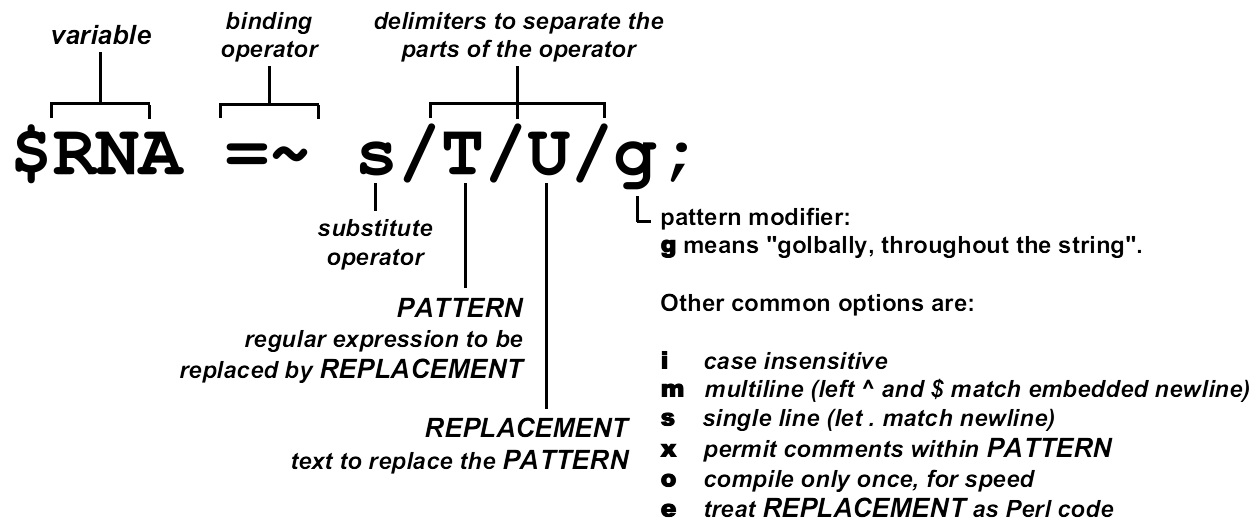
\includegraphics[width=15cm]{figure4.1.png}
  \caption{替换操作符}
  \label{fig:figure4.1}
\end{figure}

因此,这个语句含义就是“把\verb|$RNA|变量存储的字符串数据中的所有\verb|T|都替换成\verb|U|”。

替换操作符是使用正则表达式的一个例子。正则表达式对于文本处理来说至关重要,在后续的章节中你将看到,正则表达式是Perl最为强大的特性之一。

\section{使用Perl文档}
对于Perl程序员来说,最重要的资源便是Perl的文档。它应该已经安装在了你的电脑上,另外通过因特网在Perl网站上也可以找到它。对于不同的计算机系统来说,Perl文档的格式可能有少许的差别,但网络版对任何一个人来说都是一样的,这也正式我在本书中参考的版本。参看\autoref{chap:chapteraa}中的参考资料,你会找到对于Perl文档不同资源的讨论。

来试一下,让我们找找\textit{print}操作符的文档吧。首先,打开你的网页浏览器,进入 \href{http://www.perl.com}{http://www.perl.com} 网站,然后点击文档链接,依次选择“Perl的内置函数”("Perl's Builtin Functions")和“按字母顺序罗列的Perl函数”("Alphabetical Listing of Perl's Functions")。你会看到一个把Perl函数按字母顺序进行排列的一个冗长的列表。一旦你找到这个页面,你可能需要把它收藏到浏览器的书签中,因为你会频繁地访问该页面。现在点击Print来查看\verb|print|操作符的文档吧。

看一下文档中的例子,看看Perl语言的特性是如何被运用的。这往往是你找到所需内容的最快方法。

一定在你的屏幕中打开了文档,你会发现通过阅读它会找到一些答案,但也会产生其他一些疑问。文档试图以一种简洁的形式把所有的内容都包含进去,但这却会让初学者们心生胆怯。比如,\verb|print|函数文档的开头还比较简单:“打印输出一个字符串或者一个逗号分隔的字符串列表。如果成功将返回TRUE”。但之后就是一堆的胡言乱语了(在你学习的现阶段它看起来确实是这样):文件句柄?输出流?列表上下文?

文档中的所有信息都是必需的,毕竟,你需要在某个地方找到这样的全部内容!通常情况下,你可以忽略掉那些对你来说毫无意义的内容。

Perl文档中也包含了一些对学习Perl有很大帮助的教程。有时,它们会假定你掌握了比一个编程语言初学者应当掌握的知识更多的知识,但你会发现它们仍然非常有用。翻阅文档是在学习Perl语言过程中快速成长的绝佳途径。

\section{在Perl中计算反向互补}
\autoref{chap:chapter1}中已经提到了,DNA聚合物是由核苷酸构成的。考虑到DNA双螺旋中两条链的亲密关系,最好能编写这样一个程序:给出一条链,输出另一条链。这样的工作对许多生物信息学应用程序来说都是非常重要的一部分。比如,当在数据库中查询某条DNA时,常常也需要自动查询该DNA的反向互补序列,因为你手上的序列有可能是某个已知基因的负链。

回到正题,这是\autoref{exam:example4.4},它使用了一些新的Perl特性。就像你将看到的那样,它首先尝试一种方法,失败了,然后尝试另外一种方法,最终取得了成功。

%\textbf{例4-4:计算DNA一条链的反向互补链}
\lstinputlisting[label=exam:example4.4,caption={例4-4:计算DNA一条链的反向互补链}]{./scripts/example4-4.pl}

这是你屏幕上\autoref{exam:example4.4}的输出:

\begin{lstlisting}
Here is the starting DNA:

ACGGGAGGACGGGAAAATTACTACGGCATTAGC

Here is the reverse complement DNA:

GGAAAAGGGGAAGAAAAAAAGGGGAGGAGGGGA

That was a bad algorithm, and the reverse complement was wrong!
Try again ...

Here is the reverse complement DNA:

GCTAATGCCGTAGTAATTTTCCCGTCCTCCCGT

This time it worked!
\end{lstlisting}

通过从不同的末端开始读起,也就是说一条链从左向右读,另一条链从右向左读,你可以检查一下DNA的两条链是不是反向互补的。当你读这两条链的时候,比较它们对应的碱基,应该总是C和G对应、A和T对应。

在第一次尝试中,试着从原始的DNA和反向互补后的DNA中读几个字符,你会发现反向互补的第一次尝试失败了。这是一个错误的算法。

这是在你程序中经常要经历的一种体验。你写一个程序来完成某项任务,但却发现它并没有像你期望的那样工作。在这种情况下,我们需要运用已掌握的知识来尝试解决全新的问题。它并没有如期望那样完成任务,哪里出错了呢?

你会发现这样的经历会非常相似:你编写代码,但它并不工作!然后你就修正语法(这通常是最简单的,而且利用错误信息提供的线索就可以轻松修正语法),或者对问题进行思考,找到问题所在,并尝试设计一种新的可以成功的方法。通常情况下,这需要你浏览语言的文档,查找语言工作过程的细节内容,同时期望能找到一个解决问题的特性。如果这个问题在计算机上能够解决,那没你用Perl也可以将它解决。问题是,能够精确到什么程度?

在\autoref{exam:example4.4}中,计算反向互补的第一次尝试失败了。使用四个全局替换,序列中的每一个碱基都作为一个整体进行了处理。还需要另外的方法。你可以从左向右查阅DNA,每次只查找一种碱基,把它替换成互补的碱基,然后再在DNA中查找另外一种碱基,一直到字符串的结尾。然后把字符串反转过来,任务就完成了。事实上,这是一个非常好的方法,在Perl中也不难实现。但还需要学习语言的其他内容才行,这将在\autoref{chap:chapter5}中进行讲解。.

然而,在这个例子中,tr操作符——表示直译或翻译——正好适合这项任务。它看起来像替换命令一样,都使用三个正斜线来分隔不同的部分。

\textit{tr}正是我们所需要的,它会一次性把一个字符集合翻译成新的字符。\autoref{fig:figure4.2}展示了它的工作原理:需要翻译的字符集合位于前两个正斜线之间,而将要替换它们的新的字符集合则位于第二个和第三个正斜线之间。第一个集合中的每一个字符都将被翻译成第二个集合中同样位置的字符。举个例子,在\autoref{exam:example4.4}中,\verb|C|是第一个集合中的第二个字符,所以它会被翻译成第二个集合中的第二个字符,也就是\verb|G|。最后,DNA序列数据可以使用大写或者小写字母(虽然在本程序中DNA都是大写的),这两种情况在\autoref{exam:example4.4}的\textit{tr}语句中都进行了考虑。

\begin{figure}
  \centering
  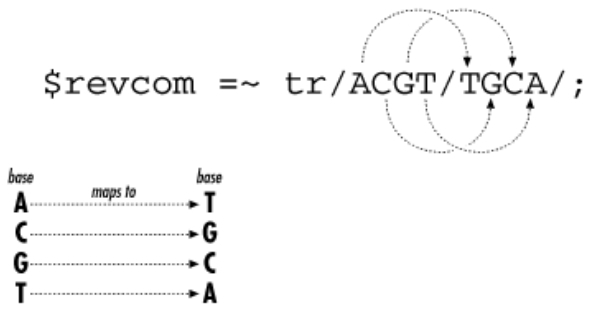
\includegraphics[width=10cm]{figure4.2.png}
  \caption{tr语句}
  \label{fig:figure4.2}
\end{figure}

\verb|reverse|函数进行的工作也是我们需要的,虽然有点大材小用了。它被设计用来反转元素的顺序,包括字符串,就像在\autoref{exam:example4.4}中看到的那样。

\section{蛋白质,文件和数组}
到现在为止,我们已经编写了处理DNA序列数据的程序,现在,我们也将要处理同样重要的蛋白质序列数据。接下来的几个小节将要学习一些新的知识,这里是一个简单的概述:

\begin{itemize}
  \item 在Perl程序中如何使用蛋白质序列数据
  \item 如何从一个文件中读入蛋白质序列数据
  \item Perl语言中的数组
\end{itemize}

在本章的剩余部分中,蛋白质和DNA序列数据都将使用到。

\section{从文件中读取蛋白质序列数据}
程序要和计算机磁盘中的文件进行交互。这些文件可以存储在任何永久性存储介质中——硬盘、光盘、软盘、Zip磁盘、磁带等。

让我们看看如何从文件中读取蛋白质序列数据吧。首先,在你的计算机上创建一个文件(使用文本编辑器),并在其中存储一些蛋白质序列数据。给这个文件起名为\textit{NM\_021964fragment.pep}(你可以在书籍网站上下载到该文件)。你将使用下列数据(人类锌指蛋白NM\_021964的一部分):

\begin{lstlisting}[language=]
MNIDDKLEGLFLKCGGIDEMQSSRTMVVMGGVSGQSTVSGELQD
SVLQDRSMPHQEILAADEVLQESEMRQQDMISHDELMVHEETVKNDEEQMETHERLPQ
GLQYALNVPISVKQEITFTDVSEQLMRDKKQIR
\end{lstlisting}

你可以给它起任意一个名字,只要和文件夹中已有的文件不重名即可。

就像好的变量名对于理解程序至关重要一样,好的文件名和文件夹名也是非常重要的。如果你有一个项目,这个项目会生成大量的文件,那你就需要认真考虑如何对这些文件和文件夹命名和组织了。不管是对于某一个研究人员还是对于一个庞大的多国团队来说,这都是非常现实的问题。花一些功夫来给文件起一个富含信息量的名字是非常重要的。

文件名\textit{NM\_021964fragment.pep}来源于蛋白质的GenBank
ID。同时,它还表明了这只是数据的一部分,而文件的后缀\textit{.pep}则提醒你文件中保存的是肽或蛋白质序列数据。当然,其他的命名方案可能会更加适合于你。不管怎样,关键的一点就是不需要打开文件,仅仅通过文件名就可以对文件保存的数据有所了解。

你已经创建或者下载了保存有蛋白质序列数据的文件,那我们就来编写一个程序吧,这个程序从文件中读入蛋白质序列数据并把它保存到变量中。\autoref{exam:example4.5}是第一次尝试,随着学习我们会逐步对它进行扩展。

%\textbf{例4-5:从文件中读取蛋白质序列数据}
\lstinputlisting[label=exam:example4.5,caption={例4-5:从文件中读取蛋白质序列数据}]{./scripts/example4-5.pl}

下面是\autoref{exam:example4.5}的输出:

\begin{lstlisting}
Here is the protein:

MNIDDKLEGLFLKCGGIDEMQSSRTMVVMGGVSGQSTVSGELQD
\end{lstlisting}

注意只有文件的第一行被打印输出出来,稍后我会解释为什么会这样。

让我们仔细研究一下\autoref{exam:example4.5}吧。在把文件名保存到\verb|$proteinfilename|变量中后,下面这个语句会打开文件:

\begin{lstlisting}
open(PROTEINFILE, $proteinfilename);
\end{lstlisting}

打开文件后,你就可以对它进行各种操作了,比如读取、写入、查找、定位到文件的特定位置、清除文件中的所有数据,等等。注意,程序假设保存在\verb|$proteinfilename|变量中的文件是存在的,而且可以打开。你将会看到如何来确认这一点,现在你可以进行一下这样的尝试:更改\verb|$proteinfilename|变量中文件的名字,这样计算机上就没有叫原来那个名字的文件了,之后运行一下程序。如果文件并不存在,你会看到一些错误信息。

如果你查阅\verb|open|函数的文档,你会看到好多选项,大多数选项都是在打开文件后让你精确指定如何使用文件的。

让我们来看一下\verb|PROTEINFILE|这个数据,它叫做\textit{文件句柄}。没有必要理解文件句柄真正是什么,它们就是你处理文件时使用的东西。对于文件句柄,比一定必须使用大写字母,但这是一个广为接受的惯例。在使用\textit{open}语句对文件句柄赋值后,对文件进行的任何交互操作都将通过使用文件句柄来进行。

使用这个语句,就可以把数据读入到程序中了:

\begin{lstlisting}
$protein = <PROTEINFILE>;
\end{lstlisting}

为什么要把文件句柄\verb|PROTEINFILE|包裹在尖括号中呢?这些尖括号叫做\textit{输入操作符}。通过把文件句柄包裹在尖括号中,你就可以从程序外部的来源中读入数据了。在这个例子中,我们读入了\verb|NM\_021964fragment.pep|文件中的数据,该文件的名字保存在\verb|$proteinfilename|变量中,而\verb|open|语句则把它和文件句柄关联了起来。数据现在就保存到了\verb|$protein|变量中,之后可以把它打印输出出来。

然而,就像我们前面已经注意到的那样,只有这个多行文件的第一行被打印了出来。这是问什么呢?因为对于读取文件还有一些知识需要学习。

有许多方法可以读取整个文件,\autoref{exam:example4.6}演示了其中的一种。

%\textbf{例4-6:从文件中读取蛋白质序列数据,第二次尝试}
\lstinputlisting[label=exam:example4.6,caption={例4-6:从文件中读取蛋白质序列数据,第二次尝试}]{./scripts/example4-6.pl}

下面是\autoref{exam:example4.6}的输出:

\begin{lstlisting}
Here is the first line of the protein file:

MNIDDKLEGLFLKCGGIDEMQSSRTMVVMGGVSGQSTVSGELQD

Here is the second line of the protein file:

SVLQDRSMPHQEILAADEVLQESEMRQQDMISHDELMVHEETVKNDEEQMETHERLPQ

Here is the third line of the protein file:

GLQYALNVPISVKQEITFTDVSEQLMRDKKQIR
\end{lstlisting}

这个程序中比较有趣的一点就是,它演示了如何成功得从文件中读取数据。每当把数据读取到\verb|$protein|这样的标量变量中后,都会对文件的下一行进行读取。上一次读取到哪儿了,现在需要读取哪一行,程序对这些信息都有所记录。

另一方面,程序的缺陷也是显而易见的。对于输入文件的每一个行,都需要编写一行代码来读入,这样太不方便了。但是,在Perl中有两个特性可以很好的解决这个问题:数据(下一小节进行介绍)和循环(参看\autoref{chap:chapter5})。

\section{数组}
在计算机语言中,数组是存储多个标量值的变量。这些标量的值可以是数字、字符串,或者,像此处的例子一样,也可以是蛋白质序列数据输入文件中的每一行。让我们看看如何来使用数组吧。\autoref{exam:example4.7}演示了如何使用数组来把输入文件中的所有行都读入进来。

%\textbf{例4-7:从文件中读取蛋白质序列数据,第三次尝试}
\lstinputlisting[label=exam:example4.7,caption={例4-7:从文件中读取蛋白质序列数据,第三次尝试}]{./scripts/example4-7.pl}

下面是\autoref{exam:example4.7}的输出:

\begin{lstlisting}
MNIDDKLEGLFLKCGGIDEMQSSRTMVVMGGVSGQSTVSGELQD
SVLQDRSMPHQEILAADEVLQESEMRQQDMISHDELMVHEETVKNDEEQMETHERLPQ
GLQYALNVPISVKQEITFTDVSEQLMRDKKQIR
\end{lstlisting}

就像你看到的,这就是文件中的全部数据。我们成功了!

使用数组的方便性显而易见——只需要一行代码就可以把所有的数据都读入到程序中了。

注意,和标量变量以美元符号(\$)起始不同,数组变量是以@符号起始的。此外,还要注意,\verb|print|函数不仅可以处理标量变量,同样可以处理数组变量。在Perl中,数组被广泛使用,所以在本书的剩余部分你会看到大量的数组应用的实例。

数组是存储多个标量值的变量。数组中的每一个项目或者元素都是标量值,可以通过在数组中的位置(它的下标或者偏移量)对它进行引用。让我们来看几个数组和数组常用操作的实例吧。我们定义一个叫做\verb|@bases|的输出,其中存储着A、C、G和T四个碱基。现在我们对它应用几个常见的数组操作。

这是一个代码片段,它演示了如何初始化数组,以及如何使用下标来访问数组中的单个元素:

\begin{lstlisting}
# Here's one way to declare an array, initialized with a list of four scalar values.
@bases = ('A', 'C', 'G', 'T');

# Now we'll print each element of the array
print "Here are the array elements:";
print "\nFirst element: ";
print $bases[0];
print "\nSecond element: ";
print $bases[1];
print "\nThird element: ";
print $bases[2];
print "\nFourth element: ";
print $bases[3];
\end{lstlisting}

这个代码片段将会输出:

\begin{lstlisting}
First element: A
Second element: C
Third element: G
Fourth element: T
\end{lstlisting}

你可以像这样把元素一个接一个的输出出来:

\begin{lstlisting}
@bases = ('A', 'C', 'G', 'T');
print "\n\nHere are the array elements: ";
print @bases;
\end{lstlisting}

它会产生这样的输出:

\begin{lstlisting}
Here are the array elements: ACGT
\end{lstlisting}

你也可以输出用空格分隔的元素(注意\verb|print|语句中的双引号):

\begin{lstlisting}
@bases = ('A', 'C', 'G', 'T');
print "\n\nHere are the array elements: ";
print "@bases";
\end{lstlisting}

它会产生这样的输出:

\begin{lstlisting}
Here are the array elements: A C G T
\end{lstlisting}

使用\verb|pop|,你可以从数组的末尾拿掉一个元素:

\begin{lstlisting}
@bases = ('A', 'C', 'G', 'T');
$base1 = pop @bases;
print "Here's the element removed from the end: ";
print $base1, "\n\n";
print "Here's the remaining array of bases: ";
print "@bases";
\end{lstlisting}

它会产生这样的输出:

\begin{lstlisting}
Here's the element removed from the end: T

Here's the remaining array of bases: A C G
\end{lstlisting}

使用\verb|shift|,你可以从数组的开头拿掉一个碱基:

\begin{lstlisting}
@bases = ('A', 'C', 'G', 'T');
$base2 = shift @bases;
print "Here's an element removed from the beginning: ";
print $base2, "\n\n";
print "Here's the remaining array of bases: ";
print "@bases";
\end{lstlisting}

它会产生这样的输出:

\begin{lstlisting}
Here's an element removed from the beginning: A

Here's the remaining array of bases: C G T
\end{lstlisting}

使用\verb|unshift|,你可以把一个元素添加到数组的开头:

\begin{lstlisting}
@bases = ('A', 'C', 'G', 'T');
$base1 = pop @bases;
unshift (@bases, $base1);
print "Here's the element from the end put on the beginning: ";
print "@bases\n\n";
\end{lstlisting}

它会产生这样的输出:

\begin{lstlisting}
Here's the element from the end put on the beginning: T A C G
\end{lstlisting}

使用\verb|push|,你可以把一个元素添加到数组的末尾:

\begin{lstlisting}
@bases = ('A', 'C', 'G', 'T');
$base2 = shift @bases;
push (@bases, $base2);
print "Here's the element from the beginning put on the end: ";
print "@bases\n\n";
\end{lstlisting}

它会产生这样的输出:

\begin{lstlisting}
Here's the element from the beginning put on the end: C G T A
\end{lstlisting}

你可以反转数组:

\begin{lstlisting}
@bases = ('A', 'C', 'G', 'T');
@reverse = reverse @bases;
print "Here's the array in reverse: ";
print "@reverse\n\n";
\end{lstlisting}

它会产生这样的输出:

\begin{lstlisting}
Here's the array in reverse: T G C A
\end{lstlisting}

你可以获取数组的长度:

\begin{lstlisting}
@bases = ('A', 'C', 'G', 'T');
print "Here's the length of the array: ";
print scalar @bases, "\n";
\end{lstlisting}

它会产生这样的输出:

\begin{lstlisting}
Here's the length of the array: 4
\end{lstlisting}

使用Perl的\verb|splice|函数,你可以在数组的任意一个位置插入一个元素:

\begin{lstlisting}
@bases = ('A', 'C', 'G', 'T');
splice ( @bases, 2, 0, 'X' );
print "Here's the array with an element inserted after the 2nd element: ";
print "@bases\n";
\end{lstlisting}

它会产生这样的输出:

\begin{lstlisting}
Here's the array with an element inserted after the 2nd element: A C X G T
\end{lstlisting}

\section{标量上下文和列表上下文}
依赖于使用的上下文环境不同,Perl的许多操作符都会有不同的表现。在Perl中有\textit{标量上下文}和\textit{列表上下文}两种上下文环境。在\autoref{exam:example4.8}对它们都进行了演示。

%\textbf{例4-8:变量上下文和列表上下文}
\lstinputlisting[label=exam:example4.8,caption={例4-8:变量上下文和列表上下文}]{./scripts/example4-8.pl}

下面是\autoref{exam:example4.8}的输出:

\begin{lstlisting}
A C G T
4
A
\end{lstlisting}

首先,\autoref{exam:example4.8}语句了一个包含四个碱基的数组。然后,赋值语句尝试把数组(它是一种列表)复制给\verb|$a|这个标量变量: 

\begin{lstlisting}
$a = @bases;
\end{lstlisting}

在这种\textit{标量上下文}中,数组会对它的大小进行求值,也就是数组中的元素数目。语句的左边是一个标量变量,这表明是一个标量上下文。

之后,\autoref{exam:example4.8}尝试把数组(重复一下,它是一种列表)赋值给另一个列表,在这个例子中,这个列表仅有\verb|$a|这么一个变量:

\begin{lstlisting}
($a) = @bases;
\end{lstlisting}

在这种\textit{列表上下文}中,数组会把它的元素展开成一个列表。语句的左边是包裹在括号中的列表,这表明是一个列表上下文。如果左侧没有足够变量用来赋值,那么将只有数组中的部分元素会被赋值给变量。Perl的这种行为在很多情况下都会出现。Perl的许多特性都被设计成在不同的上下文环境中表现出不同的行为。在\autoref{chap:chapterab}中有更多关于标量上下文和列表上文的讨论。

现在,你已经看到使用字符串和数组来保存序列和文件数据,学习了Perl的基本语法,包括变量、赋值、打印和读入文件。把DNA转录成了RNA,还计算出了DNA一条链的反向互补序列。到\autoref{chap:chapter5}的结尾,你将学习到Perl语言编程的所有基础知识。

\section{练习题}
\noindent
\textcolor{red}{\textit{习题4.1}}
\begin{adjustwidth}{2em}{}
探索编程语言对语法错误的敏感性。对于一个可以运行的程序,试着把其中任意一个语句末尾的分号删除掉,看看会产生什么样的错误信息。试着改变其他的语法项:添加一个小括号或者大括号,把“print”或其他保留字拼错,键入或者删除任何一些内容。程序员对这样的错误习以为常。即使精通语言后,在你一点点编写代码时,仍然会常常出现这样的语法错误。注意一个错误是如何导致多行错误报告的。Perl报告的出现错误的行是不是完全准确?
\end{adjustwidth}

\noindent
\textcolor{red}{\textit{习题4.2}}
\begin{adjustwidth}{2em}{}
编写一个程序,把一个整数保存到变量中并把它打印出来。
\end{adjustwidth}

\noindent
\textcolor{red}{\textit{习题4.3}}
\begin{adjustwidth}{2em}{}
编写一个把DNA(原始序列可以是大写或者小写)以小写形式(acgt)输出的程序;再编写一个把DNA以大写形式(ACGT)输出的程序。使用\textit{tr///}函数。
\end{adjustwidth}

\noindent
\textcolor{red}{\textit{习题4.4}}
\begin{adjustwidth}{2em}{}
任务和练习4.3中的一样,但这次使用\verb|\U|和\verb|\L|字符串指令符来进行大小写的转换。举个例子,\verb|print "\U$DNA"|会把\verb|$DNA|中的数据以大写形式输出出来。
\end{adjustwidth}

\noindent
\textcolor{red}{\textit{习题4.5}}
\begin{adjustwidth}{2em}{}
有时,信息也可以从RNA流向DNA。编写一个把RNA反转录成DNA的程序。
\end{adjustwidth}

\noindent
\textcolor{red}{\textit{习题4.6}}
\begin{adjustwidth}{2em}{}
读取两个文件的数据,在输出第一个文件的内容后紧接着输出第一个文件的内容。
\end{adjustwidth}

\noindent
\textcolor{red}{\textit{习题4.7}}
\begin{adjustwidth}{2em}{}
这是一个更有难度的练习题。编写一个程序,读去一个文件,然后逆序输出它的每一行,也就是首先输出它的最后一行。你可能需要看一下\textit{push}、\textit{pop}、\textit{shift}和\textit{unshift}这四个函数,从中选择一个或多个来完成此练习。你可能需要预习一下\autoref{chap:chapter5},这样就可以在程序中使用循环了。但取决于你采取的方案,这并不是必需的。或者,你可以对包含所有行的数组使用\textit{reverse}函数。
\end{adjustwidth}

